\documentclass{article}
\usepackage[]{graphicx}
\usepackage[T1]{fontenc}

\begin{document}

\graphicspath{{figures/}}


\title{von Bertalanffy growth curve for lake whitefish sample from
       southern Lake Huron in 2009}

\author{Bob Sakamano}

\maketitle

\section*{Abstract}
\label{sec:abstract}

A von Bertalanffy growth curve was fit to Lake whitefish (Coregonus
clupeaformis) sampled from southern Lake Huron in 2009.  Lake
whitefish were collected from the commerical fishery as well as the
independent survey conducted by the Ontario Ministry of Natural
resources.  A total of 111 lake whitefish were include in the sample.
The von Bertalanffy growth parameters estimated using non-linar least
squares where Linf= 600 $\pm$ 20, k = 0.25 $\pm$ 0.10, and t0= 0.1
$\pm$ 0.02.


\section*{Introduction}
\label{sec:introduction}

von Bertalanffy growth curve is often use to describe the growth of
fish.  This paper describes how a von Bertalanffy growth curve can be
fit in R and a pdf summary report can be automatically generated using
the knitr package.

\section*{Materials and Methods}
\label{sec:Materials_and_Methods}

\subsection*{The Data}
\label{sub:the_data}

Lake whitefish collected from both the commercial fishery and the
OMNR's offshore index program in 2009 were randomly selected for
inclusion in this report.  Only fish with both a fork length (mm) and
age estimate were considered to be eligible.  The sample used in is
report was created by randomly selecting up to 10 individuals from each
of the available age classes.

\subsection*{The Model}
\label{sub:the_model}

The parameters of the Von Bertalanffy growth equation where found using
non-linear least squares by fitting the following model to the
observed data:

\begin{equation}
L_i = L_{inf} (1 - e^{-k(t_i-t_0)}) + e_i
\end{equation}

$L_i$ is the length of the $i^{th}$ fish at age $t_i$, $Linf$ is the
asymptotic length (in mm), $k$ is the Brody growth coefficient, $t0$
is the theoretical length at age 0, and $e_i$  is $N(0,\sigma ^2)$.
The starting value for the asymptotic length was taken as the maximum
observed fork length in the sample, while $t0$ and $k$ were arbitrarily
set to 0.0 and 0.25 respectively.  The methods used in this analysis
closely follow those described in Quinn and Deriso (1999) and Haddon
(2001).

\section*{Results}
\label{sec:results}

A total of 111 fish were selected for this analysis.
The mean size at each age is summarized in table \ref{tbl:size-at-age}
The Von Bertalanffy model appeared to fit the data well.  Parameter
estimates and confidence intervals are presented in table
\ref{tbl:estimates} and a plot illustrating the fitted curve against
observed mean size at age has been provided in figure \ref{fig:plot_fit}.

\begin{figure}
  \begin{center} 
     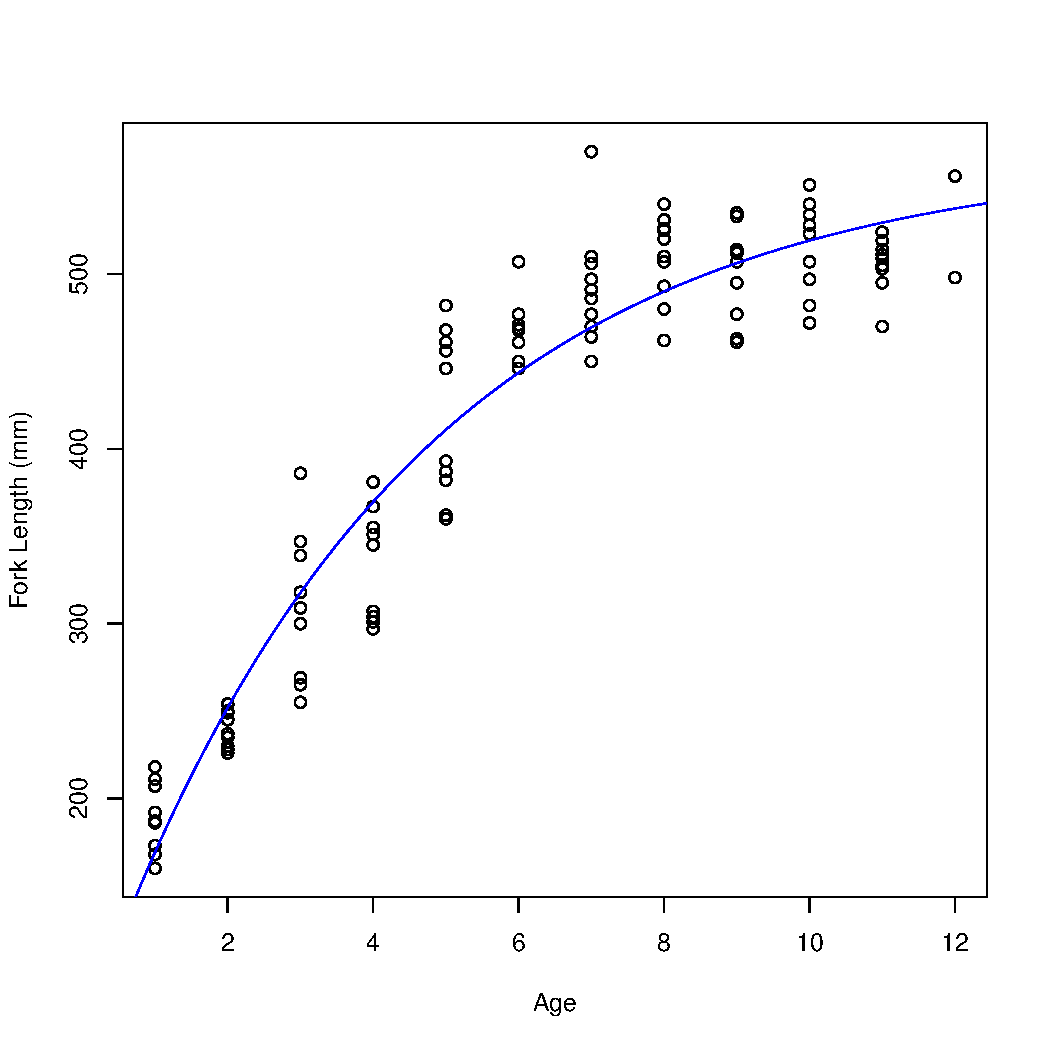
\includegraphics[width=\textwidth]{plot_fit} 
  \end{center} 
  \caption{Mean size at age of a sub-sample of lake whitefish
    collected from southern Lake Huron in 2009.  The blue line
    respresents a Von Bertalanffy growth curve fit to the data using
    non-linear least squared.}
  \label{fig:plot_fit}
\end{figure}


\begin{table}[ht]
\centering
\begin{tabular}{rrrr}
  \hline
 & Age & Observed & Predicted \\ 
  \hline
1 &   1 & 189.11 & 169.14 \\ 
  2 &   2 & 240.40 & 251.98 \\ 
  3 &   3 & 304.30 & 317.63 \\ 
  4 &   4 & 335.30 & 369.66 \\ 
  5 &   5 & 419.70 & 410.89 \\ 
  6 &   6 & 467.00 & 443.57 \\ 
  7 &   7 & 492.10 & 469.47 \\ 
  8 &   8 & 509.40 & 489.99 \\ 
  9 &   9 & 501.00 & 506.26 \\ 
  10 &  10 & 517.40 & 519.15 \\ 
  11 &  11 & 505.50 & 529.36 \\ 
  12 &  12 & 527.00 & 537.46 \\ 
   \hline
\end{tabular}
\caption{Observed and predicted size at age of lake whitefish sample from southern Lake Huron in 2009.} 
\label{tbl:size-at-age}
\end{table}



\begin{table}[ht]
\centering
\begin{tabular}{rrrrr}
  \hline
 & Estimate & Std. Error & t-value & Pr($>$$|$t$|$) \\ 
  \hline
1 & 568.38 & 15.40 & 36.92 & 0.0000 \\ 
  2 & -0.52 & 0.19 & -2.67 & 0.0088 \\ 
  3 & 0.23 & 0.02 & 9.90 & 0.0000 \\ 
   \hline
\end{tabular}
\caption{Parameter estimates, standard errors, t-values and associated p-values for Von Bertalanffy growth curve.} 
\label{tbl:estimates}
\end{table}



\section*{Discussion}
\label{sec:discussion}

Older lake whitefish are smaller than younger.  Lake whitefish from
souther Lake Huron appear to be bigger than yellow perch and smaller
than lake trout but grow slower than yellow perch and faster than lake
trout.  These findings are largely consistent with previous on Lake
Huron lake whitefish including....


\clearpage
\section*{References}
\label{sec:references}

\vspace{10 mm}

Haddon, M. Modelling and Quantitative Methods in Fisheries, Second Edition, Taylor and Francis, 2001. 424 pages.

\vspace{10 mm}

Quinn, T.J and R. B. Deriso. Quantitative Fish Dynamics, New York:Oxford Univiversity Press, 1999. 542 pages.


\end{document}
